% Created 2021-10-24 Sun 22:18
% Intended LaTeX compiler: pdflatex
\documentclass[a4paper]{article}
\usepackage[utf8]{inputenc}
\usepackage[T1]{fontenc}
\usepackage{graphicx}
\usepackage{grffile}
\usepackage{longtable}
\usepackage{wrapfig}
\usepackage{rotating}
\usepackage[normalem]{ulem}
\usepackage{amsmath}
\usepackage{textcomp}
\usepackage{amssymb}
\usepackage{capt-of}
\usepackage{hyperref}
\documentclass{article}
\usepackage{here}
\usepackage{xcolor}
\usepackage[margin=3.0cm]{geometry}
\usepackage{amsmath}
\usepackage{parskip}
\renewcommand\arraystretch{1.4}
\usepackage[margin=1in]{geometry}
\usepackage{minted}
\usepackage{multicol}
\definecolor{bg}{rgb}{0.95,0.95,0.95}
\newminted{c}{fontsize=\footnotesize,frame=single,framesep=2mm}
\usepackage[demo]{graphicx}
\usepackage{subcaption}
\usepackage{caption}
\DeclareCaptionFormat{empty}{}
\captionsetup[subfigure]{labelformat=empty}
\newminted{text}{breaklines,fontsize=\footnotesize,frame=single,framesep=2mm}
\author{Fatih Kaan Salgır - 171044009}
\date{}
\title{CSE464 - Digital Image Processing - HW1}
\hypersetup{
 pdfauthor={Fatih Kaan Salgır - 171044009},
 pdftitle={CSE464 - Digital Image Processing - HW1},
 pdfkeywords={},
 pdfsubject={},
 pdfcreator={Emacs 27.2 (Org mode 9.5)}, 
 pdflang={English}}
\begin{document}

\maketitle

\section*{Exercise 1}
\label{sec:org7e60eae}


To obtain \(A\), \(B\) can be multiplied with transformation matrix \(C\).
\begin{flalign*}
 & C \cdot B = A
\textrm{ where } C \textrm{ is }
  \begin{bmatrix}
    c_{11} & c_{12} & c_{13}\\
    c_{21} & c_{22} & c_{23}\\
    0 & 0 & 1
   \end{bmatrix} &
\end{flalign*}
Coordinates that are need to be registered by transformation matrix are;

\begin{center}
\begin{tabular}{r|l|l}
 & B(x,y) & A(x,y)\\
\hline
1 & 1,2 & 2,2\\
2 & 2,1 & -1,4\\
3 & 3,1 & -4,-4\\
\end{tabular}
\end{center}

Multiplication of each point in image B, gives the point in image A.
\begin{flalign*}
 C \cdot B_1 &= A_1 & \\
 C \cdot B_2 &= A_2 & \\
 C \cdot B_3 &= A_3 &
\end{flalign*}

For \(B_1\);
\begin{flalign*}
& \begin{bmatrix}
    c_{11} & c_{12} & c_{13}\\
    c_{21} & c_{22} & c_{23}\\
    0 & 0 & 1
   \end{bmatrix}
\cdot
 \begin{bmatrix}
    1 \\
    2 \\
    1
   \end{bmatrix}
=
 \begin{bmatrix}
    2 \\
    2 \\
    1
   \end{bmatrix}
  &
\end{flalign*}
\begin{flalign*}
    c_{11} + 2c_{12} + c_{13} &= 2 &\\
    c_{21} + 2c_{22} + c_{23} &= 2 &
\end{flalign*}

For \(B_2\);
\begin{flalign*}
& \begin{bmatrix}
    c_{11} & c_{12} & c_{13}\\
    c_{21} & c_{22} & c_{23}\\
    0 & 0 & 1
   \end{bmatrix}
\cdot
 \begin{bmatrix}
    2 \\
    1 \\
    1
   \end{bmatrix}
=
 \begin{bmatrix}
    -1 \\
    4 \\
    1
   \end{bmatrix}
  &
\end{flalign*}
\begin{flalign*}
    2c_{11} + 2c_{12} + c_{13} &= -1 &\\
    2c_{21} + c_{22} + c_{23} &= 4 &
\end{flalign*}


For \(B_3\);
\begin{flalign*}
& \begin{bmatrix}
    c_{11} & c_{12} & c_{13}\\
    c_{21} & c_{22} & c_{23}\\
    0 & 0 & 1
   \end{bmatrix}
\cdot
 \begin{bmatrix}
    3 \\
    1 \\
    1
   \end{bmatrix}
=
 \begin{bmatrix}
    -4 \\
    4 \\
    1
   \end{bmatrix}
  &
\end{flalign*}
\begin{flalign*}
    3c_{11} + 2c_{12} + c_{13} &= -4 &\\
    3c_{21} + c_{22} + c_{23} &= 4 &
\end{flalign*}

Using first equations (\(c_{1i}\)) obtained by the matrix multiplication;
\begin{flalign*}
    c_{11} + 2c_{12} + c_{13} &= 2 &\\
    2c_{11} + c_{12} + c_{13} &= -1 &\\
    3c_{11} + c_{12} + c_{13} &= -4 &
\end{flalign*}
\begin{flalign*}
    c_{11} &= -3 &\\
    c_{12} &= 0 &\\
    c_{13} &= 5 &
\end{flalign*}

Using second equations (\(c_{2i}\)) obtained by the matrix multiplication;
\begin{flalign*}
    c_{21} + 2c_{22} + c_{23} &= 2 & \\
    2c_{21} + c_{22} + c_{23} &= 4 & \\
    3c_{21} + c_{22} + c_{23} &= 4 &
\end{flalign*}
\begin{flalign*}
    c_{21} &= 0 &\\
    c_{22} &= -2 &\\
    c_{23} &= 6 &
\end{flalign*}

The transformation matrix \(C\) is;
\begin{flalign*}
C
&= \begin{bmatrix}
    -3 & 0 & 5\\
    0 & -2 & c_{23}\\
    0 & 0 & 1
   \end{bmatrix}
  &
\end{flalign*}



\newpage
\section*{Excercise 2}
\label{sec:org325ea50}

Morphological opening is used to remove artifacts while preserving the main object.

It is experimented with \(Z_4\) and \(Z_8\) structuring elements. While \(Z_4\) left a single artifact, \(Z_8\) successfully removed all the artifacts. However, on the edge areas of the image such as hands and legs, \(Z_4\) was better compared to \(Z_8\) in terms of preserving the main object.

\begin{figure}[htp]
\centering
\begin{subfigure}{.33\textwidth}
  \centering
  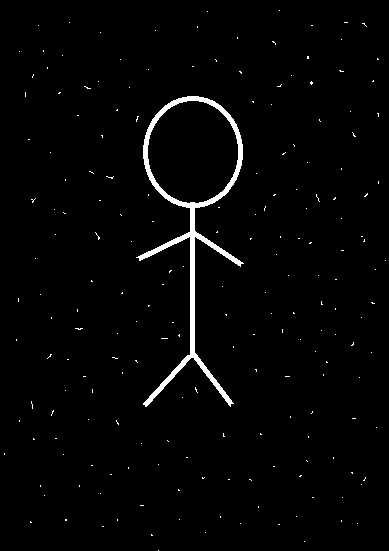
\includegraphics[width=.9\linewidth]{Image1.png}
  \caption{Original image}
  \label{fig:sub1}
\end{subfigure}%
\begin{subfigure}{.33\textwidth}
  \centering
  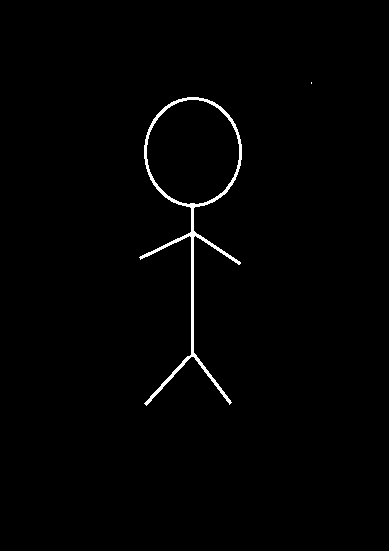
\includegraphics[width=.9\linewidth]{ex2-erosion-z4.png}
  \caption{Eroded image using $Z_4$}
  \label{fig:sub2}
\end{subfigure}
\begin{subfigure}{.33\textwidth}
  \centering
  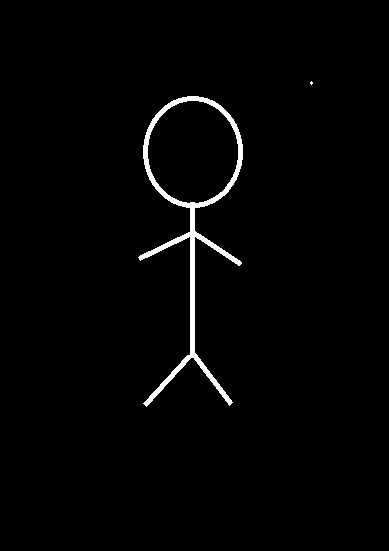
\includegraphics[width=.9\linewidth]{ex2-dilation-z4.png}
  \caption{Dilated image using $Z_4$}
  \label{fig:sub2}
\end{subfigure}
\caption{Morphological opening with $Z_4$ structuring elemnet}
\label{fig:test}
\end{figure}


\begin{figure}[htp]
\centering
\begin{subfigure}{.33\textwidth}
  \centering
  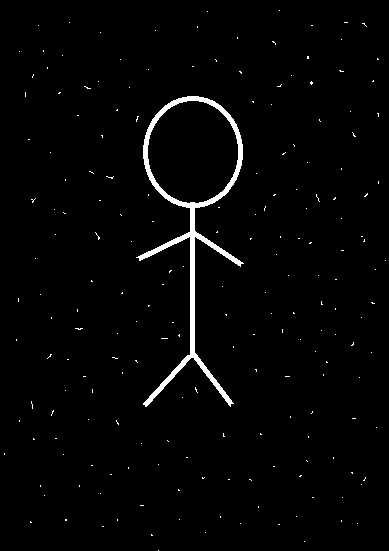
\includegraphics[width=.9\linewidth]{Image1.png}
  \caption{Original image}
  \label{fig:sub1}
\end{subfigure}%
\begin{subfigure}{.33\textwidth}
  \centering
  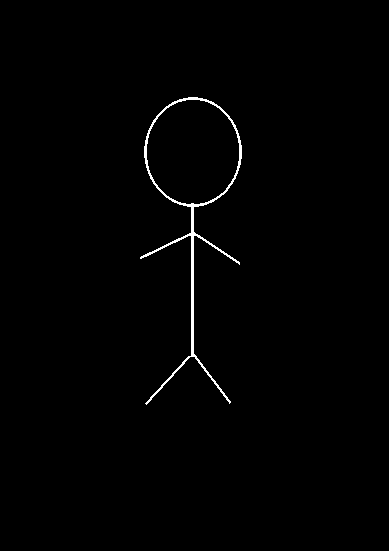
\includegraphics[width=.9\linewidth]{ex2-erosion-z8.png}
  \caption{Eroded image using $Z_8$}
  \label{fig:sub2}
\end{subfigure}
\begin{subfigure}{.33\textwidth}
  \centering
  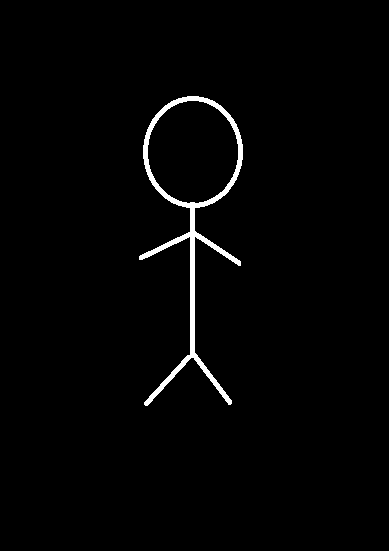
\includegraphics[width=.9\linewidth]{ex2-dilation-z8.png}
  \caption{Dilated image using $Z_8$}
  \label{fig:sub2}
\end{subfigure}
\caption{Morphological opening with $Z_8$ structuring elemnet}
\label{fig:test}
\end{figure}



\newpage
\section*{Excercise 3}
\label{sec:orge0213d8}

\(8\times8\) cross structuring element is used to erode the image. To make the curve intersections stand out, the image is dilated with \(17\times17\) ellipse structuring element. Negation of the original image is summed with the intersection points, to separate curve segments. Lastly, connected component labeling can be applied in order to count number of curve segments. However, there are some errors near the edges of the image.


\begin{figure}[htp]
\centering
\begin{subfigure}{.5\textwidth}
  \centering
  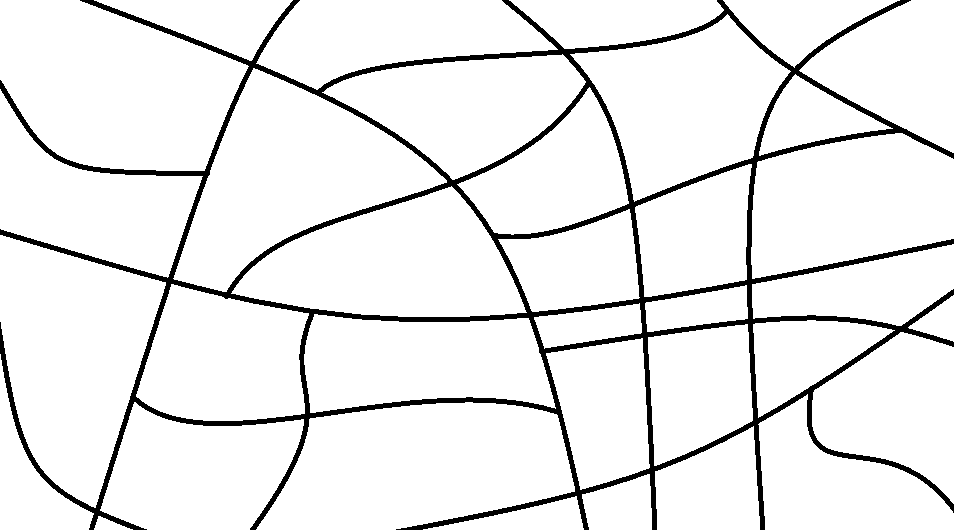
\includegraphics[width=.9\linewidth]{Image2}
  \caption{Original image}
  \label{fig:sub1}
\end{subfigure}%
\begin{subfigure}{.5\textwidth}
  \centering
  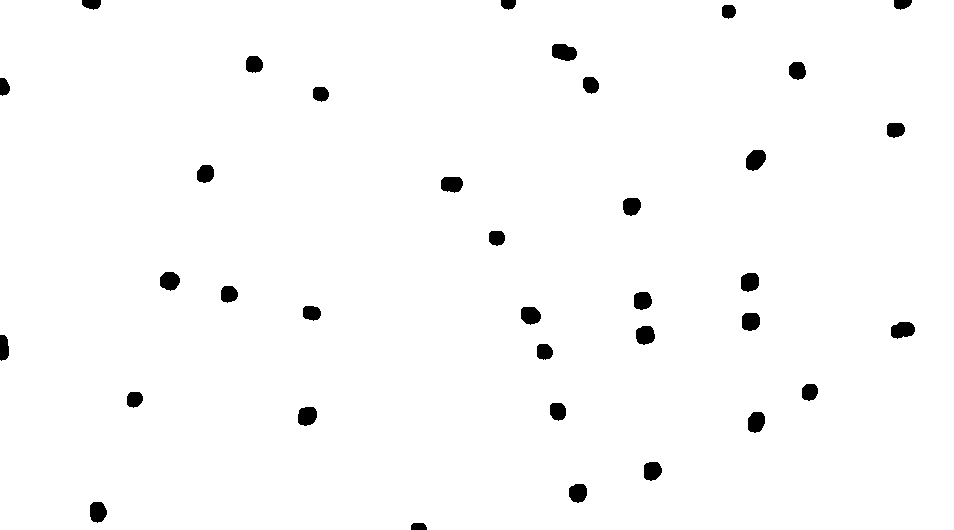
\includegraphics[width=.9\linewidth]{ex3.2}
  \caption{After applying erosion followed by dilation}
  \label{fig:sub2}
\end{subfigure}
\captionsetup{format=empty}
\label{fig:test}
\end{figure}

\begin{figure}[htp]
\centering
\begin{subfigure}{.5\textwidth}
  \centering
  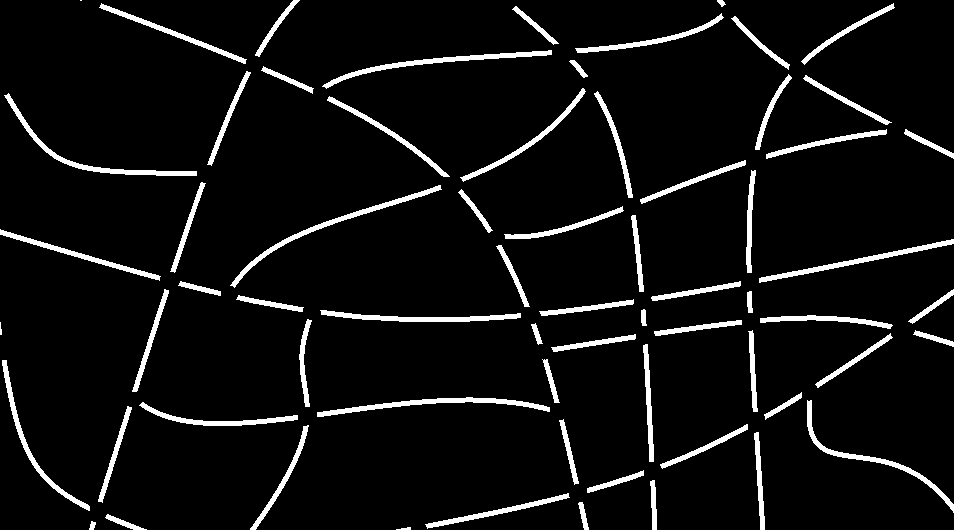
\includegraphics[width=.9\linewidth]{ex3.3}
  \caption{Seperated curve segments}
  \label{fig:sub1}
\end{subfigure}%
\begin{subfigure}{.5\textwidth}
  \centering
  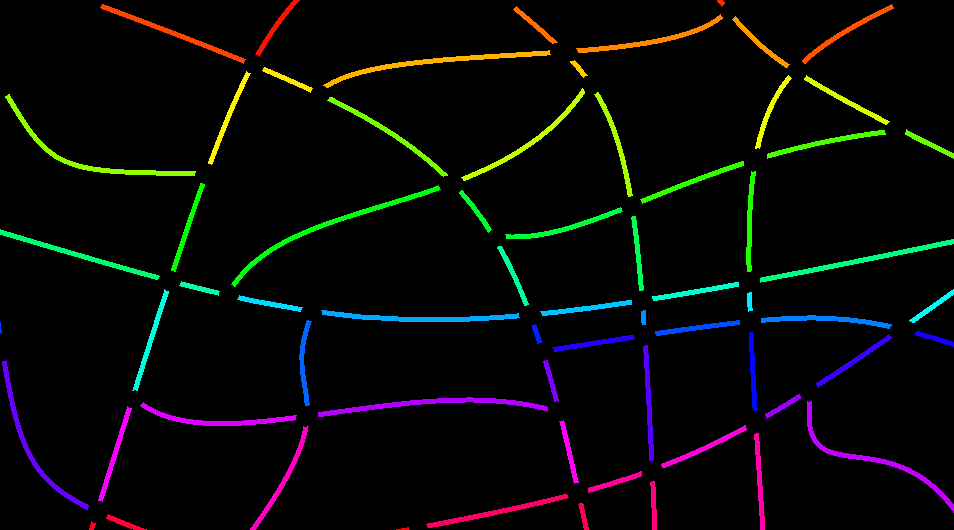
\includegraphics[width=.9\linewidth]{ex3.4}
  \caption{Curve segments colored using CC labeling}
  \label{fig:sub2}
\end{subfigure}
\captionsetup{format=empty}
\label{fig:test}
\end{figure}



\newpage
\section*{Exercise 4}
\label{sec:org8afe074}

One of the teeth of the hair comb is used as a structuring element. The image is inverted (negated) and morphological opening is applied. This allows detecting the faultless teeth of the comb. Then the opened version of the images is arithmetically summed with the original version of the image in order to detect the faulty teeth. To make the missing teeth more distinguishable, the image is dilated by \(4 \times 4\) structuring element. The last image demonstrates the missing teeth over the original one.

\begin{figure}[htp]
\centering
\begin{subfigure}{.33\textwidth}
  \centering
  
\includegraphics[width=.9\linewidth]{Image3b}
  \caption{Original image}
\end{subfigure}%
\begin{subfigure}{.33\textwidth}
  \centering
  
\includegraphics[width=.9\linewidth]{ex4.1-negated}
  \caption{Negated image}
\end{subfigure}
\begin{subfigure}{.33\textwidth}
  \centering
  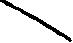
\includegraphics[width=.5\linewidth]{kernelex}
  \caption{Custom structuring element ($73\times43$ px)}
\end{subfigure}
\captionsetup{format=empty}
\end{figure}
\begin{figure}[htp]

\centering
\begin{subfigure}{.33\textwidth}
  \centering
  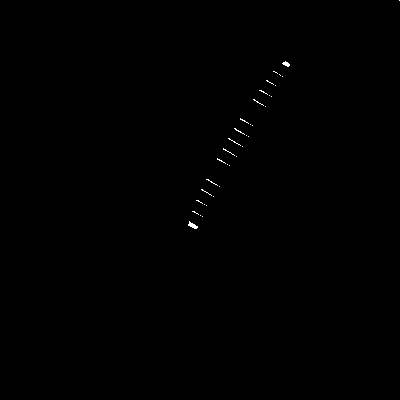
\includegraphics[width=.9\linewidth]{ex4.2-erosion}
  \caption{Eraded version of the negated image with custom SE}
  \label{fig:sub1}
\end{subfigure}%
\begin{subfigure}{.33\textwidth}
  \centering
  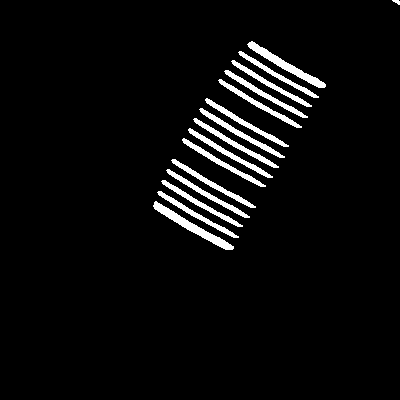
\includegraphics[width=.9\linewidth]{ex4.3-opening}
  \caption{Dilation is applied (opened)}
  \label{fig:sub2}
\end{subfigure}
\begin{subfigure}{.33\textwidth}
  \centering
  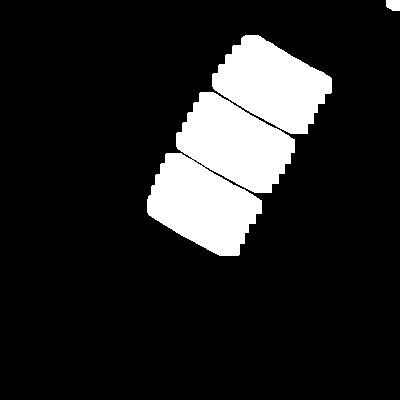
\includegraphics[width=.9\linewidth]{ex4.4-dilated}
  \caption{Dilation with SE = $13\times 13$}
  \label{fig:sub2}
\end{subfigure}
\captionsetup{format=empty}
\label{fig:test}
\end{figure}

\begin{figure}[htp]
\centering
\begin{subfigure}{.33\textwidth}
  \centering
  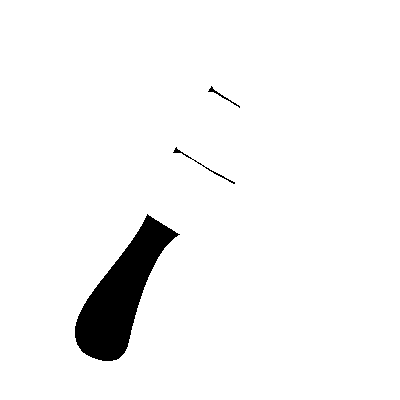
\includegraphics[width=.9\linewidth]{ex4.5-img-dilated}
  \caption{Summation with original image}
  \label{fig:sub1}
\end{subfigure}%
\begin{subfigure}{.33\textwidth}
  \centering
  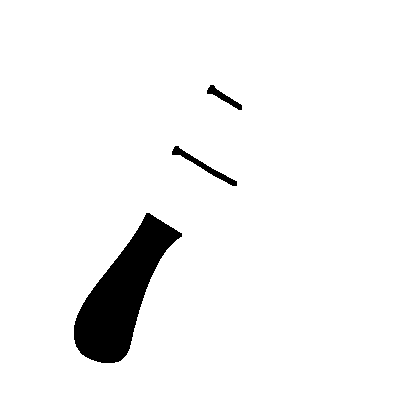
\includegraphics[width=.9\linewidth]{ex4.6-eroted}
  \caption{Dilated with SE = $4 \times 4$}
  \label{fig:sub2}
\end{subfigure}
\begin{subfigure}{.33\textwidth}
  \centering
  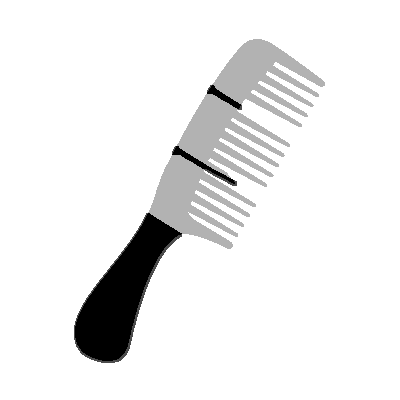
\includegraphics[width=.9\linewidth]{ex4.7-weighted}
  \caption{Demonstration of final result}
  \label{fig:sub2}
\end{subfigure}
\captionsetup{format=empty}
\label{fig:test}
\end{figure}
\end{document}
